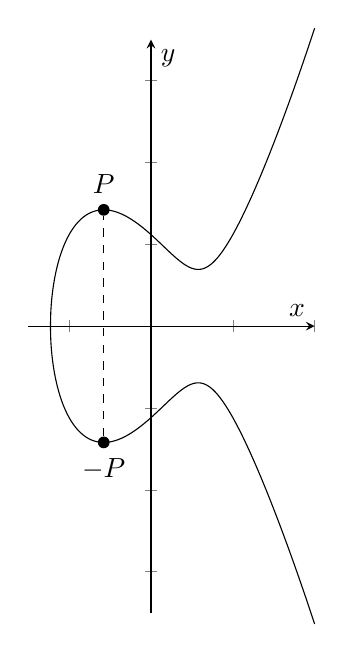
\begin{tikzpicture}
    \begin{axis}[
        xmin=-3,
        xmax=4,
        ymin=-7,
        ymax=7,
        xlabel={$x$},
        ylabel={$y$},
        scale only axis,
        axis lines=middle,
        % set the minimum value to the minimum x value
        domain=-2.456678:4,      % <-- works for pdfLaTeX and LuaLaTeX
        samples=1000,
        smooth,
        % to avoid that the "plot node" is clipped (partially)
        clip=false,
        % use same unit vectors on the axis
        axis equal image=true,
        xticklabels={,,},
        yticklabels={,,}
    ]
        \addplot [black] {sqrt(x^3-4*x+5)};
        \addplot [black] {-sqrt(x^3 - 4*x + 5)};
        
         % Some math constant macros
        \pgfmathsetmacro\localmaximum{-2/sqrt(3)}       
       	% add nodes to the points and the corresponding labels
       	\node [label={$P$}, circle,fill,inner sep=1.5pt] (P) at (\localmaximum, 2.842) {};
		\node [label=below:{$-P$}, circle,fill,inner sep=1.5pt] (-P) at (\localmaximum, -2.842) {};
       	\draw [black, dashed] (-P) -- (P);
    \end{axis}
\end{tikzpicture}